\documentclass{article}
\usepackage[utf8]{inputenc}
\usepackage{graphicx}
\usepackage{amsmath}
\usepackage{hyperref}
\usepackage[a4paper, textwidth=450pt]{geometry}

\graphicspath{ {./data/} }

\title{EP Homework 6}
\author{Adam Kit}
\date{19 May 2020}


\begin{document}

\maketitle
\section{Superposition}
We are tasked with finding the probability density $|\psi |^2$ for the superposiition of two stationary wavefunctions
\begin{equation}
\psi = C_1 \psi_1 + C_2 \psi_2
\label{wavefunction}
\end{equation}
When we take the norm of Equation \ref{wavefunction}, we get the following:

\begin{equation}
|\psi |^2 = |C_1 \psi_1 + C_2 \psi_2 |^2 = |C_1 \psi_1 |^2 + |C_2 \psi_2 |^2 + C_1^*C_2 \psi_1^* \psi_2 + C_1 C_2^* \psi_1 \psi_2^*
\label{wfprob}
\end{equation}
where in \ref{wfprob} the star represents the complex conjugate. \\ As seen in Figure \ref{superposition1}, when $\psi_1$ and $\psi_2$ correspond to different atomic states, n=3 and n=4 respectively, the superposition is as one expects. The Wave Functions are simply added together, while the probabilities are a combination of the two. So depending on the atomic states of the two wave functions that are superimposed, the density and wavefunction are converging towards the larger n.


\begin{figure}
  \centering
  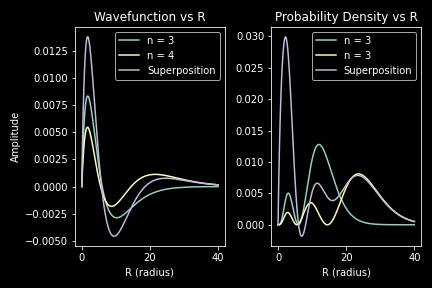
\includegraphics[scale=0.8]{superposition1.png}
  \caption{Radial Wave function $\psi (r)$ and Probability $|\psi (r) |^2$ }
  \label{superposition1}
\end{figure}
\section{Potential Step 1 }
If the section is not filled in at time of submission, it means I did not finish the problem 2 in the homework. My initial thoughts are to solve the two regions with certain $E < U_0 $ and prove that photons are emitted with energy $E_{photon} = U_0$
\section{Potential Step 2 }

In the lecture notes we discuss both sides of this potential wall problem, however here we have the potential defined by:
\[
U(x) =
  \begin{cases}
    \text{0,} &\quad\text{if x $<$ }\text{0} \\
    \text{$U_0$,} &\quad\text{if x}\ge\text{0}
  \end{cases}
\]

The 1D time independent Schroedinger Equation we aim to solve is:
\begin{equation}
i \hbar \frac{\partial}{\partial t }\psi = -\frac{\hbar^2}{2m} \frac{\partial^2}{\partial x^2} \psi + U(x) \psi
\label{schro}
\end{equation}

The solution for $\psi (x)$ has the following form for Region 1:
\begin{equation}
\psi_{I} = A e^{ikx} + B^{-ikx}
\label{region1}
\end{equation}

and for Region 2:
\begin{equation}
\psi_{II} = C e^{\alpha x} + D^{-\alpha x}
\label{region2}
\end{equation}

Where $\alpha = \sqrt{\frac{2m(U_0 - E)}{\hbar^2}}$

One can note now, that for each $\psi$, there is both a forward propogating wave and a backwarg propogating wave, yet in our problem, only region II has both forward and backward components, while region I has only the transmitted (forward).
Thus Eq \ref{region1} becomes:
\begin{equation}
\psi_I = Ae^{ikx}
\label{region1.1}
\end{equation}

And with continuity conditions
$$\psi_I(x=0) = \psi_{II}(x=0)$$

and
$$\frac{d \psi_I}{dx}_{x=0} =\frac{d \psi_{II}}{dx}_{x=0}  $$

We find the system of equations when inserting $x = 0$ into Eqs: \ref{region1.1} and \ref{region2} and their first order derivitaives:

\begin{equation}
C + D = A
\label{condition1}
\end{equation}

and
\begin{equation}
\alpha(C - D) = ikA
\label{condition2}
\end{equation}

The coeffeicients are then found to be, when C = 1:
\begin{equation}
D = \frac{\alpha - ik}{\alpha + ik}
\end{equation}
\begin{equation}
A = 1 + D = 1 + \frac{\alpha - ik}{\alpha + ik} = \frac{2\alpha}{\alpha + ik}
\end{equation}
So the probability for reflection is:
$$ P_{reflection} = R = |D|^2 = (\frac{\alpha-ik}{\alpha + ik})^2 $$
and
$$ P_{transmission} =  1 - P_{reflection} = T =  \frac{4\alpha ik}{(\alpha + ik)^2}$$
These are the same as the fresnel coefficients for normal incidence, except the refractive indexes of the regions are replaced by the Total Energy in both regions, i.e $n_2 = \alpha $ and $n_1 = ik$

\end{document}
